\section{Motivación}

El mundo del transporte experimentó un fuerte cambio a principios del siglo XX. Desde entonces, la acción de conducir ha acompañado el día a día de muchas personas hasta hoy. Sin embargo, con el paso del tiempo, esta relación se ha ido deteriorando, cambiando la percepción de conducir de un placer a una obligación. Factores como los atascos, el estrés o la actitud de otros conductores, influyen negativamente en el estado del conductor, dando lugar a situaciones peligrosas propensas al error humano.  Por otro lado, una conducción insegura deriva en un mayor consumo de combustible y un aumento del 15 \% de las emisiones de \ce{CO2} a la atmósfera, según el Instituto de la Diversificación y Ahorro de la Energía (\cite{energetica}), perjudicando directamente al medioambiente. Si bien es cierto que la tendencia actual es sustituir los combustibles fósiles por las energías renovables, en el mundo de la automoción todavía existen barreras económico-sociales que ralentizan esta transición.

La conducción autónoma aporta una solución parcial a estos problemas, proyectando un futuro más seguro y amigable para los usuarios de las carreteras. El desarrollo de sistemas inteligentes en vehículos ha supuesto un gran avance tecnológico en la industria, facilitando al conductor tareas como la evaluación del entorno y la toma de decisiones. 

En los últimos años, la caracterización del entorno de navegación ha sido el principal foco en la optimización de la conducción autónoma. La redundancia de sensores y las comunicaciones entre vehículos e infraestructura pueden ayudar a la prevención de situaciones críticas donde el conductor deba asumir el control del vehículo en el menor tiempo posible. Sin embargo, las corrientes más conservadoras clasifican de futuristas estas tecnologías, ya que la única realidad plausible a día de hoy es la del tráfico mixto, donde encontrar vehículos de niveles de autonomía no superiores a 2 en entornos abiertos y de niveles 3-4 en espacios controlados. Parte de esta ralentización se debe al largo proceso de implementación por parte de las legislaciones en diferentes países del mundo, sin olvidar la aceptación de la propia sociedad y las barreras tecnológicas. A pesar de los múltiples estudios y ensayos realizados, la confiabilidad en estos sistemas se ve cuestionada, debido en gran parte a que muchos de los accidentes que se producen en conducción autónoma podrían ser fácilmente evitables en conducción manual. Por un lado, las validaciones de los sistemas basados en sensores obtienen en una alta tasa de éxito en entornos cerrados, pero no terminan de contemplar todas las situaciones que podrían darse en el mundo real, como es el estado de una carretera deteriorada o el comportamiento impredecible de otro vehículo. Por otro, el reconocimiento del entorno para una persona no solo se basa en el sistema visual, también intervienen elementos como el sonido ambiental, las sensaciones, la intuición y los prejuicios, que permiten realizar predicciones que conforman la toma de decisiones en conducción (Figura \ref{fig:1.1}).

\newpage

\begin{figure}[ht]
  \centering
  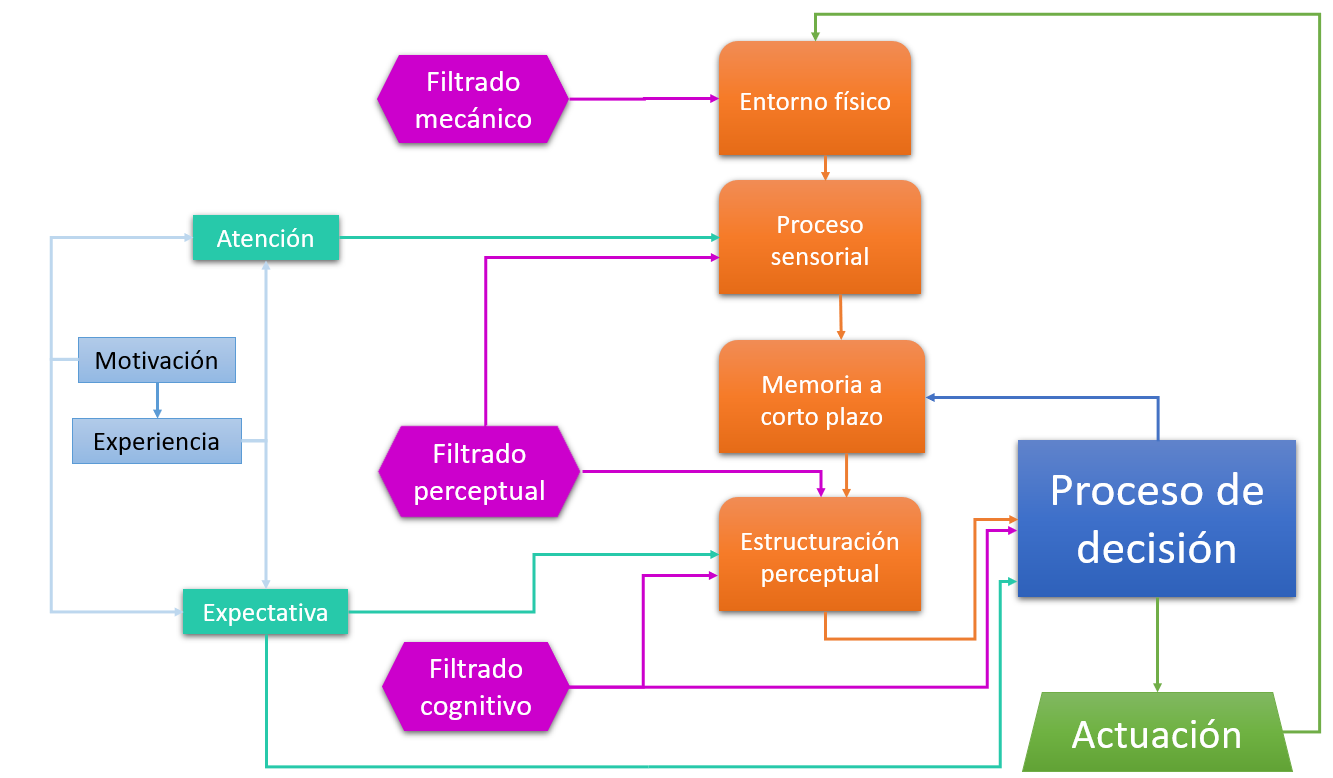
\includegraphics[width=12.5cm]{figures/1.1.png}
  \caption{\label{fig:1.1} Diagrama de las variables que intervienen en el proceso de decisión.}
\end{figure}

Estudiar el comportamiento del conductor proporciona información relevante en los procesos cognitivos empleados en la realización de una tarea, como son el orden de prioridades en el análisis del entorno, los tiempos de respuesta o los recursos mentales disponibles frente a estímulos. Es por ello por lo que numerosas empresas de vehículos con opciones de conducción parcialmente automatizada, se sienten abiertas a instalar sensores hacia el interior del habitáculo, con objeto de comprobar la atención del conductor en caso de aparecer un evento crítico. Numerosos fabricantes ya implementan sistemas basados en cámaras para detectar estados de somnolencia y fatiga, como Ford (Monitoring System), Toyota (Driver Monitoring System), Volkswagen (Fatigue Detection System), Mercedes-Benz (Attention Assist) y Volvo (Driver Alert Control) entre otros. La importancia de estos sensores reside en los primeros niveles de autonomía, donde el conductor es el principal supervisor y tiene la responsabilidad de retomar el control cuando la situación lo requiera. En la misma línea se observa que los procesos automatizados suelen derivar en un exceso de confianza por parte del supervisor, produciendo fenómenos como la hipovigilancia y el amodorramiento, que pueden ser evitables gracias a estos sensores. 

El dilema en la determinación de un evento crítico es el tiempo que invierte el sistema en identificarlo y darle el control al conductor. Una alta capacidad de cálculo en la detección debe complementarse con una buena identificación. A pesar de que los conductores humanos no son tan rápidos como un algoritmo matemático, este podría predecir un peligro con mayor antelación, valorando otros criterios no matemáticos y siendo el tiempo final de respuesta menor. Algunos algoritmos de toma de decisiones están basados en inteligencia artificial, con el fin de replicar las capacidades humanas de decisión. Sin embargo, no son capaces de crear razonamientos en base a situaciones que no se hayan definido previamente. Garantizar el máximo de reglas en el sistema de decisiones es determinante para poder tener un buen sistema de navegación.  

La caracterización del comportamiento del conductor es una parte importante en el desarrollo de los algoritmos de conducción, tanto a nivel individual como grupal. Las decisiones no solo dependen de variables espacio-temporales constantes, sino que la disposición del entorno y el comportamiento de los vehículos adyacentes pueden generar variabilidad en dichos parámetros. Además, una conducta eficiente y ordenada no es realista, ya que la conducción es un medio flexible, donde puede existir un lenguaje y una comunicación no verbal previa a la realización de ciertas maniobras. Debido a ello, un vehículo autónomo en tráfico mixto podría enfrentarse a situaciones de inadaptabilidad, al no comprender las intenciones de los demás vehículos o realizar acciones inesperadas. 

La comprensión de las decisiones humanas puede ser estudiada mediante el sistema visual, ya que es uno de los principales receptores de información relevante del entorno. Los movimientos oculares, al igual que el de la cabeza, son un reflejo de la estrategia atencional seguida, permitiendo determinar patrones en la ejecución humana de ciertas maniobras. Estudiar el proceso de resolución humano ante una situación demandante contribuye directamente a una mejora en la identificación de eventos críticos y a la elaboración de reglas en el sistema de decisión. En esta Tesis Doctoral se propone analizar la influencia de la complejidad del entorno sobre las variables atencionales del conductor, con el fin de elaborar algoritmos de toma de decisiones naturalistas que ayuden a la integración de la conducción autónoma en el tráfico mixto. 

\section{Objetivos}

El objetivo de esta Tesis se centra en aportar una solución a la integración de los vehículos autónomos en el tráfico mixto, a través de una mejora en la caracterización del comportamiento del conductor. La optimización del proceso de toma de decisiones, sobre el que se asientan los algoritmos implementados en vehículos autónomos, contribuye directamente en la resolución de situaciones imprevistas durante la conducción. Por ello, el objetivo principal es comprender la interpretación del entorno por parte de un conductor humano y desarrollar un modelo de toma de decisiones para vehículos autónomos a partir de esa interpretación. Observando las variables atencionales se puede determinar la estrategia atencional seguida, contribuyendo en el desarrollo de algoritmos de toma de decisiones naturalistas.

Al mismo tiempo se alcanzan los siguientes objetivos secundarios, los cuales son abordados en los tres capítulos que comprenden esta Tesis:

\begin{itemize}
  \item Analizar la influencia de las variables atencionales en maniobras complejas en vías de alta capacidad, como son autovías y autopistas, y el comportamiento del conductor ante diferentes niveles de asistencia en la conducción autónoma.
  \item Integrar el sistema de percepción del conductor con la fusión sensorial de detección del entorno, utilizando tecnologías de seguimiento ocular, láser 3D y visión artificial.
  \item Proponer, ajustar y validar un modelo determinista para la toma de decisiones aplicado a la conducción autónoma en base a diferentes niveles de información disponible. 
\end{itemize}

Las maniobras propuestas se resumen en incorporaciones, cambios de carril y adelantamientos, diferenciándose estas dos últimas en el rebase del vehículo delantero. Todos los ensayos experimentales se realizan en tráfico real, en contextos interurbanos, utilizando vehículos equipados con tecnología propia de la conducción autónoma. 

\section{Estructura de la tesis}

La presente Tesis Doctoral se estructura en los siguientes capítulos, como se describe a continuación.

El \hyperref[ch1]{Capítulo 1} corresponde a estas primeras páginas, sirviendo como \emph{Introducción} a dicho escrito y presentando las motivaciones y los objetivos que se pretenden alcanzar en esta investigación.
El \hyperref[ch2]{Capítulo 2} presenta el \emph{Estado de la cuestión}, mostrando mediante literatura los desarrollos existentes sobre los que se apoya la presente Tesis. Partiendo de los modelos de comportamiento existentes en la conducción se profundiza en las variables habitualmente utilizadas y los sensores a través de los cuales pueden ser obtenidas. Los desarrollos y las aportaciones de la Tesis Doctoral se presentan en los capítulos 3, 4 y 5. 
En el \hyperref[ch3]{Capítulo 3} se plantea la utilización de \emph{Variables atencionales} en la conducción, en concreto en los modelos de toma de decisiones. Se muestran dos apartados principales, concernientes a las maniobras de incorporación y adelantamiento en niveles de conducción parcialmente automatizada, donde se estudia la información proporcionada por el sistema de seguimiento visual en relación al estado del conductor y las estrategias atencionales empleadas en la realización de la maniobra. 
En el \hyperref[ch4]{Capítulo 4} se realiza una \emph{Fusión sensorial} entre el sistema de percepción del conductor, compuesto por el de seguimiento visual y el de captación del movimiento de la cabeza, y dos sistemas de percepción del entorno, constituidos por una cámara y un sensor láser, determinando los obstáculos que el conductor mira durante la conducción. 
El \hyperref[ch5]{Capítulo 5} propone el desarrollo de un algoritmo para un \emph{Modelo de toma de decisiones en conducción autónoma} con objeto de mejorar el naturalismo de los modelos de comportamiento. Este capítulo se completa con los resultados obtenidos de los capítulos anteriores, gracias a los cuales el modelo será ajustado y validado utilizando datos de ensayos experimentales en conducción real.
Por último, se presentan las \hyperref[ch6]{Conclusiones y líneas de investigación futuras} junto a la \hyperref[ch7]{Difusión de resultados} en revistas y congresos de índole nacional e internacional concernientes a la Tesis Doctoral. 

